\section{Subgraphs of the Comparability Grid}

\begin{frame}{Proving Comparability Grid Universality}
Strategy: Embed $\Grid$ in $\CGrid$. Two ways to do this:

\[
\begin{tikzpicture}[x=1cm,y=1cm]
	\node[font=\Large] (cgrid) at (0,2.8) {$\CGrid$};
	\node[font=\Large] (grid) at (0,0) {$\Grid_{m \times n}$};
	\draw[->,thick,bend right=35] (cgrid) to node[midway,left=14pt,align=center,text width=3.8cm]
		{\only<2->{\textbf{Method 1}\\What grids can we get from vertex deletion?}} (grid);
	\draw[->,thick,bend right=35] (grid) to node[midway,right=14pt,align=center,text width=3.8cm]
		{\only<3->{\textbf{Method 2}\\How can we embed $\Grid_{m \times n}$ in $\CGrid$?}} (cgrid);
\end{tikzpicture}
\]

\end{frame}

\begin{frame}{$\Grid_{2 \times n}$ is a subgraph}

\begin{lemma}
For all $n \in \mathbb{N}$, $\Grid_{2 \times n}$ is a subgraph of a sufficiently large $\CGrid$.
\end{lemma}

\begin{proof}<2->

\begin{center}
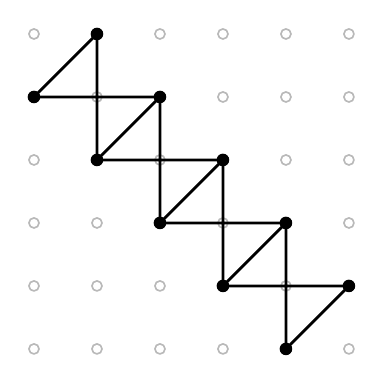
\begin{tikzpicture}[scale=0.8, line cap=round, line join=round]

\foreach \x in {0,...,5} {
    \foreach \y in {0,...,5} {
    \draw[gray!55, line width=0.6pt] (\x,\y) circle[radius=0.08];
    }
}

\draw[black, line width=1.0pt]
    (0,4)--(1,5)
    (1,5)--(1,4)
    (0,4)--(1,4)--(2,4)
    (1,4)--(1,3)
    (1,3)--(2,4)
    (1,3)--(2,3)--(2,4)
    (2,3)--(2,2)
    (2,3)--(3,3)
    (2,2)--(3,3)
    (2,2)--(3,2)--(3,3)
    (3,2)--(3,1)
    (3,2)--(4,2)
    (3,1)--(4,2)
    (3,1)--(4,1)--(4,2)
    (4,1)--(4,0)
    (4,1)--(5,1)
    (4,0)--(5,1);

\foreach \p in {(0,4),(1,5),(1,3),(2,4),(2,2),(3,3),(3,1),(4,2),(4,0),(5,1)}{
    \fill[black] \p circle[radius=0.10];
}

\end{tikzpicture}
\end{center}
\end{proof}

\end{frame}

\begin{frame}{Which grids are subgraphs?}

\begin{theorem}
$\Grid_{k \times n}$ is not a subgraph of any  $\CGrid$ for $k > 2$, $n > 2$.
\end{theorem}

\begin{proof}<2->
Using a computer, we enumerate all possible $9$ vertex subgraphs of $\CGrid$. No such subgraph is isomorphic to $\Grid_{3 \times 3}$.
\end{proof}

\end{frame}